% !TeX program = lualatex
% !TeX encoding = utf8
% !TeX root = ../Thermod.tex

%=========================================================
\Opensolutionfile{answer}[\currfilebase/\currfilebase-Answers]
\Writetofile{answer}{\protect\section*{\nameref*{\currfilebase}}}
\chapter{Основні поняття. \mbox{Нульовий закон термодинаміки}}\label{\currfilebase}
\makeatletter
\def\input@path{{\currfilebase/}}
\makeatother
%=========================================================







%% --------------------------------------------------------
\section{1}
%% --------------------------------------------------------


Термодинаміка вивчає закони теплового руху в рівноважних системах (класична термодинаміка) та узагальнює ці закони на нерівноважні системи (термодинаміка незворотних процесів). Термодинаміка вивчає поведінку \emph{макроскопічних систем}, просторові розміри яких значно більші ніж характерні розміри молекул, а час існування достатній для проведення необхідних вимірів \emph{макроскопічних параметрів}, що характеризують систему та її відношення до довколишніх тіл (густина, об'єм, тиск, намагніченість і т.д.). Питання про відношення даної системи до розгляду термодинаміки мають вирішуватися окремо в кожному конкретному випадку. Насправді, чи мають термодинаміка або\emph{ статистична фізика}  вивчати поведінку молекули ДНК, яка складається з мільйонів частинок? В будь-якому разі термодинаміка займається динамічними системами з дуже великою кількістю степенів волі.

Користуючись механістичним підходом такі системи можуть бути розглянуті шляхом розв'язування дуже великою кількості рівнянь руху з підстановкою не меншої кількості початкових умов. Наприклад, моль газу, який містить число Авогадро ($ 6.022\cdot10^{23} $) частинок --- потребує в три рази більше рівнянь руху, що є зовсім нереальним хоча б за кількістю паперу та чорнил, які потрібно витратити (Ландау). На щастя, стан системи можна описати невеликою кількістю макроскопічних параметрів, рівноважні значення яких можуть бути пораховані методами статистики на основі визначеної моделі молекулярної будови речовини, або визначені експериментально.

Термодинаміка постулює деякі положення, перевірені віковою працею людства й підтверджувані знову та знову, та на їх основі вивчає властивості рівноважних систем та закони наближення до рівноваги. Перейдемо до розгляду деяких важливих понять.

\emph{Термодинамічною системою} будемо називати частину Всесвіту, що вивчається (рис.~\ref{pic:ThermodSysA}).

%=========================================================
\begin{figure}[h!]\centering
%---------------------------------------------------------
    \begin{subcaptionblock}{0.45\linewidth}\centering
        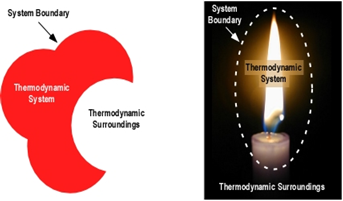
\includegraphics[width=\linewidth]{Lec1/ThermodSysA}
        \caption{Термодинамічна система і її оточення (термостат)}\label{pic:ThermodSysA}
    \end{subcaptionblock}
\quad%---------------------------------------------------------
    \begin{subcaptionblock}{0.45\linewidth}\centering
        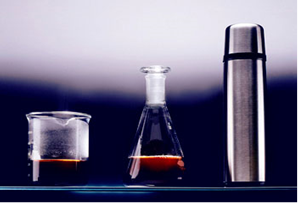
\includegraphics[width=\linewidth]{Lec1/ThermodSysB}
        \caption{Приклад відкритої, закритої та ізольованої системи (зліва направо)}\label{pic:ThermodSysB}
    \end{subcaptionblock}
%---------------------------------------------------------
\caption{}
\end{figure}
%=========================================================

\emph{Термостатом} (\emph{термодинамічним оточенням}) називається та частина повної системи, яка не розглядається, але обмежує систему по деякій реальній або віртуальній границі. Вважається, що термостат вносить деякі умови до системи, що вивчається.


Системи бувають (рис.~\ref{pic:ThermodSysB}):
\begin{itemize}
    \item ізольованими --- зовсім не взаємодіють з навколишнім середовищем, хіба що механічно або через поле;
    \item замкнутими --- не має обміну речовиною з термостатом;
    \item відкритими ---  можливий обмін як енергією так і речовиною.
\end{itemize}


Макроскопічні параметри розподіляють на \emph{зовнішні} та \emph{внутрішні}. До перших відноситься об’єм, так як визначається положенням зовнішніх предметів, напруженість магнітного поля, тому що залежить від положення джерел поля. Усі величини, що визначаються положенням та рухом частинок, які входять у систему, називаємо \emph{внутрішніми}. З останнього витікає, що різниця між внутрішніми та зовнішніми параметрами визначається границею між системою та навколишнім середовищем.

З макроскопічних параметрів можна виділити термодинамічні змінні. Вибрана належним чином, сукупність термодинамічних змінних повністю визначає систему в тому сенсі, що інші величини є їх функціями.

Макроскопічні параметри розподіляють на інтенсивні та екстенсивні. До перших відносять величини, що не залежать від розмірів системи (тиск, температура). Величини, що змінюються пропорційно до маси, при її умовному розподіленні на частини, відносять до екстенсивних (енергія, об’єм, ентропія і т. д.). За Гегелем принципова відмінність між ними пояснюється способом вимірів. Екстенсивні величини можна порівняти зі схожими (однорідними). Наприклад, довжину з еталоном довжини. Для інтенсивних це зробити не можливо та потрібна деяка функціональна залежність між інтенсивною величиною та набором екстенсивних. Наприклад, не має еталона температури, але останню можна знайти вимірявши висоту стовпчика у термометрі.

Сукупність незалежних макроскопічних параметрів, що характеризують систему, визначає її \emph{стан}. Існують фізичні величини (макроскопічні параметри), які не залежать від попередніх умов та повністю визначаються станом системи в даний момент (тиск, температура, магнітне поле). Їх називають \emph{функціями стану}. Стан системи називають стаціонарним, якщо він не змінюється з часом. Крім того, якщо в системі відсутні стаціонарні потоки енергії або речовини, то стан системи називається \emph{рівноважним}. Саме такими системами й займається класична термодинаміка.





%% --------------------------------------------------------
\section{2}
%% --------------------------------------------------------

\emph{Термодинамічна рівновага} це стан до якого кінець кінцем приходить будь-яка ізольована система, якщо її залишити саму по собі. Пояснюючи це поняття зауважимо, що в стані т.д. рівноваги відсутній макроскопічний рух у напрямку системи: переміщення, потік енергії частинок. Це не означає, що в цьому стані відсутній будь-який рух. Напроти, в цьому стані продовжується мікроскопічний рух частинок. Наш повсякденний досвід свідчить, що стан системи задовільно описується  макроскопічними параметрами, які є усередниними характеристиками мікроскопічного руху. Наприклад, тиск газу на стінки посудини приблизно дорівнює квадрату імпульсу частинок газу.


Дослід показує, що два тіла, які знаходяться у контакті один з одним кінець кінцем приходять до стану теплової рівноваги. Це твердження постулюється термодинамікою та, за виразом Фаулера, отримало назву нульового закону термодинаміки. З нього витікає закон транзитивності теплової рівноваги. Е Дійсно, якщо тіла $\mathcal{A}$, $\mathcal{B}$, $\mathcal{C}$ з'єднати у вигляді кільця, так щоб кожне з них дотикалось двох інших, то теплова рівновага встановиться в місцях дотику $\mathcal{AB}$, $\mathcal{AC}$ та $\mathcal{BC}$, бо в іншому випадку загальна рівновага ну була би можливою, що протирічить результатам дослідів.





%% --------------------------------------------------------
\section{3}
%% --------------------------------------------------------


Поняття <<теплота>>, сенс якого і має визначити термодинаміка, з'являється з почуття різниці між теплим та холодним при дотику до тіла: але кількісна, задовільна для науки міра теплового стану не може бути виведена з почуття, яке дає низькоякісний і суб'єктивний за визначення результат. Задля цієї мети користуються іншим явищем, яке згідно з дослідом, спостерігається у більшості тіл збільшення об'єму одночасно з нагріванням  --- і, на основі якого, і будують прилад для визначення температури  термометр. Пояснити дію такого приладу дозволяє нульовий закон термодинаміки, а саме закон транзитивності. Отже, якщо одне з тіл $\mathcal{A}$, $\mathcal{B}$, $\mathcal{C}$ (наприклад $\mathcal{B}$) вважати пробним, то за результатом зрівняння стану тіла $\mathcal{A}$ та $\mathcal{B}$ , та окремо $\mathcal{B}$ та $\mathcal{C}$, можна зробити висновок про наявність або можливість теплової рівноваги між $\mathcal{A}$ та $\mathcal{C}$, навіть якщо останні технічним шляхом привести у контакт неможливо (наприклад вершину г.~Монблан та 1 корпус КПІ). Таким чином тіло $\mathcal{B}$ умовимося вважати тим тілом, за допомогою якого й будемо вивчати тепловий рух.

Математично ці твердження виглядають так. Нехай стан системи $\mathcal{A}$
характеризується незалежними параметрами $\alpha_{\mathcal{A}}$.
Не обмежуючи загальності, вважаємо, що
$\alpha_{\mathcal{A}} = \{P_{\mathcal{A}}, V_{\mathcal{A}}\}$ і
аналогічно $\mathcal{B}$, $\mathcal{C}$ характеризуються $\alpha_{\mathcal{B}} = \{P_{\mathcal{B}}, V_{\mathcal{B}}\}$ та $\alpha_{\mathcal{C}} = \{P_{\mathcal{C}}, V_{\mathcal{C}}\}$. Якщо $\mathcal{A}$ та $\mathcal{B}$ у стані термодинамічної рівноваги, то між $\mathcal{A}$ та $\mathcal{B}$ існує співвідношення:
\begin{equation}\label{eq:F3}
    F_3 (P_{\mathcal{A}}, V_{\mathcal{A}}, P_{\mathcal{A}},V_{\mathcal{A}}) = 0.
\end{equation}

Аналогічно, для пар $ВС$ та $АС$ маємо:
\begin{equation}\label{eq:F1}
    F_1  (P_{\mathcal{C}}, V_{\mathcal{C}} ,P_{\mathcal{B}},V_{\mathcal{B}})=0
\end{equation}
та
\begin{equation}\label{eq:F2}
    F_2  (P_{\mathcal{A}},V_{\mathcal{A}}, P_{\mathcal{C}}, V_{\mathcal{C}} )=0
\end{equation}

Розв'язуючи \eqref{eq:F3} та \eqref{eq:F1} відносно $P_B$ отримаємо:
\begin{equation}\label{eq:PB}
    P_{\mathcal{B}} = \phi_1 (P_{\mathcal{C}}, V_{\mathcal{C}}, V_{\mathcal{B}})=\phi_3 (P_{\mathcal{A}}, V_{\mathcal{A}}, V_{\mathcal{B}})
\end{equation}
Це є еквівалентом \eqref{eq:F2} і, відповідно,  не повинно залежати від $\mathcal{B}$, так як не залежить від $P_{\mathcal{B}}$ рівновага між $\mathcal{A}$ та $\mathcal{C}$.

Звідси співвідношення \eqref{eq:PB} еквівалентно:
\begin{equation}\label{eq:f1}
    f_1 (P_{\mathcal{C}},V_{\mathcal{C}})=f_3 (P_{\mathcal{A}}, V_{\mathcal{A}}).
\end{equation}

Діючи у такий спосіб отримаємо:

\begin{align}
    f_2 (P_{\mathcal{B}}, V_{\mathcal{B}})=f_3 (P_{\mathcal{A}}, V_{\mathcal{A}}), \\
    f_1 (P_{\mathcal{C}}, V_{\mathcal{C}})=f_2 (P_{\mathcal{B}}, V_{\mathcal{B}}).
\end{align}

Звідси витікає, що величина $\theta = f(P, V)$ може бути зручною мірою для визначення стану рівноваги або температурою за деякою шкалою --- емпіричною температурою. Цю особливість відбиває походження назви температури від латинської \emph{temperatus} (спокійний, врівноважений). Очевидно, що кожна \emph{монотонна} функція від $\theta$ також може бути названа температурою. Побудований таким чином прилад дозволяє нам встановлювати рівність температур тіл, проте не більше. Для того щоб поняття «велика та мала» температура мало визначений фізичний сенс та, притому, тим який приписується цим поняттям, будемо вважати, що тіло $\mathcal{A}$ має більшу температуру за тіло $\mathcal{B}$, якщо при зведені їх до теплового контакту, тіло $\mathcal{A}$ охолоджується, а тіло $\mathcal{B}$ натомість нагрівається. В цьому сенсі \emph{температура є мірою нагрітості тіла}.

Очевидно, температура це величина інтенсивна та для її кількісного визначення потрібно використати функціональну залежність $\theta = f(P, V)$. Вибір на користь визначення об'єму або тиску можна зробити саме з огляду на зручність, головне, щоб при цьому інша змінна залишалась постійною. Задля того, щоб вимірювана температура не залежала від того, яку величину ми вимірюємо, за необхідністю вимірюють відносні зміни, наприклад $\frac{\Delta P}{P_0}$  або  $\frac{\Delta V}{V_0}$. Звідси витікає, що ці зміни певної властивості \emph{робочої речовини термометра}, співставляємо із такою в характерному стані \emph{еталонної речовини}, наприклад точки танення льоду, що легко визначається навіть неозброєним оком. Щоб визначити шкалу термометра, необхідно вибрати ще один характерний стан речовини та приписати йому іншу температуру. Наприклад, таким станом може бути кипіння води. Приписуючи відносній зміні об’єму $\frac{[\delta V_{100}]}{V_0}$  в цьому стані число «$100$», а в стані плавлення льоду $\frac{[\delta V_{0}]}{V_0}$ , відповідно «$0$», та розділюючи різницю показань на $100$ одиниць, отримуємо одиницю виміру температури $t = 1^\circ$C. Подібним чином можна побудувати й інші емпіричні шкали, як це зробили Фарангейт, Ньютон, Реомер та інші. Згідно з методом побудови такого приладу зовсім не обов'язково вимірювати об'єм або тиск. Це може бути наприклад, густина випромінювання розжареного об'єкта. Важливо, щоб ця характеристика була \emph{функцією стану системи}. На практиці використовують й інші термометри, дія яких базується на існуванні функціонального зв'язку між деякою властивістю робочої речовини та температурою. Наприклад, $R=R(t)$  або $\mathcal{E}_(\text{e.p.c.})=\mathcal{E}(t)$.





%% --------------------------------------------------------
\section{4}
%% --------------------------------------------------------





Методом, розібраним вище, був побудований  один з перших термометрів  газовий. Це стало можливим завдяки особливо простому взаємозв'язку між тиском створюваним газом, його об'ємом та ступенем його нагрітості. Робертом Бойлем, сучасником Ньютона, було встановлено, а в подальшому Едмоном Маріоттом було підтверджено, що між тиском та об’ємом певної кількості газу існує співвідношення:
\begin{equation}\label{eq:pv}
    pv = \theta = \mathrm{const},
\end{equation}
де стала $\theta$, крім як від природи газу залежить і від емпірично вимірюваної температури $t$. Ще більш разючим виявилось відкриття Жака Шарля, в подальшому наново відкрите Гей-Люсаком. Згідно з ним різні гази, особливо ті, що важко зріджуються, такі як водень, кисень, азот, шляхетні гази при награванні від $0$ до $1$ градуса емпіричного термометра розширюються на величину приблизно рівну $\alpha=1/273$ частини первинного об'єму, якщо вибравши $1$ градус згідно:
\begin{equation}
    1^\circ\text{C} = \frac{v_1 - v_0}{v_{100} - v_0} 100,
\end{equation}
де $v_0$ об’єм, що займає газ при $t=0$, а $v_{100}$ об’єм при $t=100$. Тоді отримаємо:
\begin{equation}
    v-v_0=\alpha t v_0,
\end{equation}
або
\begin{equation}\label{eq:v}
    v=v_0 (1+\alpha t).
\end{equation}

Приймемо для $t = 0^\circ$C, що справедливо $pv_0=\theta_0$. Помноживши $p$ на \eqref{eq:v}, із урахуванням \eqref{eq:pv} отримаємо:
\begin{equation}\label{eq:theta}
    \theta = pv = \theta_0 (1+\alpha t).
\end{equation}

Зручно змістити довільно вибрану температуру $t=0$ на $\alpha^{-1}$ й ввести нову температурну шкалу $T=t+\alpha^{-1}$. Тоді \eqref{eq:theta} набуває вигляду:
\begin{equation}\label{eq:theta2}
    pv = \theta_0T
\end{equation}

В новій температурній шкалі, плавлення льоду відбувається при $t=273.15^\circ\text{С} \approx \alpha^{-1}$.

Отримане співвідношення дозволяє побудувати як термометр постійного об'єму, так і термометр постійного тиску. Це пояснює причини за якими тиск досі вимірюється в торах --- тиск, що створюється стовбцем ртуті в $1$~мм. Наведемо також інші одиниці виміру тиску:
\begin{align*}
    1\ \text{Па}  &= \frac{\text{Н}}{\text{м}^2},\\
    1\ \text{бар} &= 10^5\ \text{Па}\ \text{(стовб води в $10$ м)},\\
    1\ \text{атм} &= 760 \text{мм. рт. ст.} = 760\ \text{торр.} = 101.325\ \text{кПа}.
\end{align*}

Побудований таким чином термометр з такою шкалою отримав назву ідеально-газового, оскільки формально згідно \eqref{eq:theta2}, об’єм, що займає газ при $T = 0$, повинен дорівнювати нулеві. Звичайно, таких газів у природі не існує, однак домовимося користуватися таким термометром, вважаючи можливим його заповнити газом при нескінченно низькому тиску. Слід сказати, що точність термометра, заповненого реальним газом, в більшості випадків буде нас задовольняти (Таблиця~\ref{tab:gase_thermometers}).

\begin{table}[!htbp]\centering
    \caption{Виправлення до показників газових термометрів}\label{tab:gase_thermometers}
    \begin{tblr}{
    colspec = {X[c, m]X[c, m]X[c, m]X[c, m]}
    }
    \toprule
    $t^\circ$C   & \ce{He}     & \ce{H2}  & \ce{N2}  \\
    \midrule
    $200^\circ$  & $+0.002$    & $+0.020$ & $+0.132$ \\
    $100^\circ$  & $0$         & $0$      & $0$      \\
    $0^\circ$    & $0$         & $0$      & $0$      \\
    $-100^\circ$ & $+0.006$    & $0,052$  & $0,399$  \\
    \bottomrule
    \end{tblr}
\end{table}

Для остаточного з’ясування  взаємозв’язку $P$, $V$ та $T$ необхідно  встановити значення $v_0$. У $1811$ році Амадео Авогадро висловив гіпотезу про те, що при одних і тих самих температурі та тиску рівні об'єми газів містять рівну кількість молекул. Окремим наслідком цього твердження є відомий закон, згідно з яким, один моль будь-якого газу при 0oC та $P=760$~торр займає $22.4$~л. Знаючи це, легко знайти невідому константу та отримати:
\begin{equation}
    PV = \nu RT = \frac{M}{\nu} RT
\end{equation}
де $\nu$ --- кількість молів, а $ R= 8.311441$ $\frac{\text{Дж}}{\text{К}\cdot\text{моль}}$ --- універсальна газова стала. Цей вираз отримав назву рівняння Клапейрона-Менделєєва. В окремому випадку при $P=\mathrm{const}$ закон називають рівнянням Гей-Люсака, а при $V=\mathrm{const}$ --- рівнянням Амундсена.





%% --------------------------------------------------------
\section{5}
%% --------------------------------------------------------




Отриманий вираз є ні чим іншим, як рівнянням стану для ідеальних або майже ідеальних газів і задовільно описує їх поведінку при невеликому тиску та помірних температурах. Реальні гази часто порушують виведену закономірність. На теперішній час тільки для газів відомо близько $150$ емпірично встановлених \emph{термічних рівнянь стану}. Найбільш простим з них є \emph{рівняння Ван-дер Ваальса}, що правдиво відтворює поведінку газів навіть при їх переході до стану рідини:
\begin{equation}\label{eq:VanDerVaals}
    \left(p + \frac{a}{v^2}\right)(v - b) = RT.
\end{equation}

Ще більш точнішими є \emph{перше} та \emph{друге рівняння Дітерічі}, \emph{рівняння Бертло}, а також \emph{віріальне розвинення}:
\begin{equation}\label{eq:virial}
        pv = RT \left(1 + \frac{A}{v} + \frac{B}{v^2} + \frac{C}{v^3} + \ldots \right).
\end{equation}

Не слід думати , що термодинаміка обмежується лише вивченням поведінки газів. Безумовно для інших речовин (рідин або твердих тіл) рівняння стану має записуватися по іншому. В більшості випадків вони встановлюються емпіричним шляхом і тільки для доволі спрощених моделей можуть бути отримані методами статистичної фізики. Так для тіла, яке знаходиться при достатньо низьких температурах в кристалічному стані за певних припущень Дебаєм був отриманий наступний вираз:
\begin{equation}\label{eq:Debay}
    pv + v \frac{d\Phi}{dv} = - \frac{d''\ln''\theta}{d''\ln''v}\ \frac35 \pi^4 R\Theta \left(\frac{T}{\Theta}\right)^4.
\end{equation}
де $\Phi$ залежить від потенціалу взаємодії між молекулами, $\Theta$ параметр, що визначається кристалічною структурою та має розмірність температури (температура Дебая). Формула правдива при $T \ll \Theta$. Як ще один приклад термічного рівняння стану наведемо рівняння стану для газу фотонів (випромінювання, яке знаходиться в тепловій рівновазі зі стінками об’єму, в якому воно міститься). Рівняння може бути отримано теоретично:
\begin{equation}\label{eq:Stef-Boltz}
    P = \sigma \frac{T^4}{3},
\end{equation}
де $\sigma$ --- стала Стефана-Больцмана. Зазначимо, що в даному випадку залежність від $V$ відсутня. Термічне рівняння стану не обов'язково є функціональним зв'язком $P$, $V$ та $T$. Набір незалежних термодинамічних змінних може бути різноманітним та визначається характером явища, що досліджується. Так для парамагнетичних речовин (мідь, алюміній ,повітря) зв'язок встановлюється між намагніченістю $M$, полем $H$ та температурою $T$. Згідно з законом Вейса:
\begin{equation}
    M = \chi \frac{H}{T},
\end{equation}
де $\chi$ --- магнітна сприятливість речовини. Тим не менше, кожне термічне рівняння стану пов’язує температуру, який-небудь внутрішній параметр ($P$, $M$, \ldots) та якийсь із зовнішніх ($V$, $H$, \ldots).

Окрім термічного рівняння стану існує ще калорічне рівняння стану, що пов’язує енергію, температуру та будь-який зовнішній параметр. Особливо простим таке рівняння є для ідеального газу:
\begin{equation*}
    U = C_V T.
\end{equation*}

Для твердих тіл при $T \ll \Theta$ воно також виглядає просто:
\begin{equation*}
    U = \alpha V T^4,
\end{equation*}
де $\alpha$ --- деяка стала.  Зрештою для газу фотонів:
\begin{equation*}
    U = \sigma V T^4.
\end{equation*}

В загальному випадку сумарна кількість рівнянь стану дорівнює числу незалежних макроскопічних параметрів, що описує стан системи. Важливо, що для термодинаміки зовсім не має значення звідки вони отримуються. Якщо вони відомі, то за допомогою термодинамічного методу можна встановити всі термодинамічні властивості системи.



%% --------------------------------------------------------
\section{6}
%% --------------------------------------------------------




Розглянемо яким чином можна змінити стан термодинамічної системи. По-перше між самою системою та оточуючим її середовищем слід встановити \emph{термодинамічний контакт}. Останній прийнято розподіляти на $3$ типи:

\begin{itemize}
    \item \emph{Механічна взаємодія} має місце якщо система або над системою здійснюється робота за допомогою механічних сил або полів ( електромагнітного, гравітаційного ). В цьому випадку термостат розглядають як джерело роботи.

    \item \emph{Теплова взаємодія} здійснюється у формі передачі тепла за допомогою теплопровідності або теплової радіації. Термостат виконує роль теплового резервуару або теплової бані.

    \item \emph{Матеріальна взаємодія} спричиняє обмін частинками між системою та термостатом і останній вважають джерелом або резервуаром частинок.
\end{itemize}

Термодинаміка розглядає тільки такі зміни стану при якому початковий або кінцевий стан є рівноважними. Щиро кажучи, ситуація ідеалізована так як, наприклад, для здійснення роботи над газом, необхідно, як показано на рисунку, щоб $P_e > P_i$, тому як мінімум для зміни стану системи має бути динамічна взаємодія. Однак, при належно підготовленому експерименті, $\delta P$ завжди можна вибрати менше ніж наперед задана будь-яка мала величина, та якомога ближче наблизитися  до рівноважного процесу.

Процеси, при яких різниця між кінцевим та початковим станом нескінченно мала називають \emph{інфінітезимальними}. Якщо при цьому система та термостат увесь час залишаються в рівновазі, то процес називають квазістатичним. Такий процес завжди є \emph{оборотнім}, так як оборотній процес проходить через таку саму послідовність рівноважних станів, що й прямий. Розрізняють \emph{ізотермічний} ($T = \mathrm{const}$), \emph{ізобаричний} ($P = \mathrm{const}$),  \emph{ізохоричний} ($V = \mathrm{const}$) та адіабатичний квазістатичний процеси. Останній вимагає існування лише механічного контакту між системами.


Не слід думати, що при адіабатичному процесі система завджи термічно ізольована від термостату. На практиці достатньо, щоб процеси передачі тепла між системами ( теплопровідність, радіація ) протікали набагато повільніше ніж характерний час зміни параметрів системи. Наприклад, якщо процес \emph{циклічний}, тобто початковий та кінцевий стан збігаються, то період за який система повертається в вихідний стан повинен бути набагато менше ніж час дисипації енергії.




%% --------------------------------------------------------
\section{7}
%% --------------------------------------------------------




Найбільш очевидним способом зміни стану системи є здійснення над системою роботи. Прийнято вважати роботу додатною, якщо вона здійснюється системою над зовнішніми тілами (оточенням) та від’ємною в протилежному випадку. При нескінченно малій рівноважній (квазістатичній) зміні зовнішнього параметра системи хi, робота визначається як:
\begin{equation*}
    \delta A = F_i dx_i,
\end{equation*}
де $F_i$ --- спряжена зовнішньому параметру узагальнена сила, яка завжди є внутрішнім параметром та в рівновазі є функцією зовнішніх параметрів та температури. У випадку здійснення роботи рідиною або газом, для яких тиск в усьому об'ємі який вони займають є однаковим, робота, що здійснюється системою при розширені від $V$ до $V+dV$ складається із елементарних робот $Pd\sigma dx$, де $d\sigma$ --- елементарні площадки, на які умовно розіб'ємо поверхню $S$ об’єму, що займає газ або рідина. В результаті:
\begin{equation}\label{eq:delta A}
    \delta A = \sum\limits_i\delta A_i = p \sum\limits_i d\sigma_i dx_i = p dV.
\end{equation}


Повна робота, що здійснюється газом або рідиною при зміні об’єму від $V_1$ до $V_2$, розраховується інтегруванням виразу \eqref{eq:delta A} в цих границях. Наприклад, $1$~моль газу, який задовольняє рівнянню стану ідеального газу та розширюється ізотермічно від $V_1$ до $V_2$, здійснює роботу:
\begin{equation*}\label{eq:2a}\tag{2а}
    A = \int\limits_{V_1}^{V_2} p dV = RT  \int\limits_{V_1}^{V_2} \frac{dV}{V} = RT \ln\left(\frac{V_2}{V_1}\right).
\end{equation*}

Геометричний сенс цього інтегралу --- площа під кривою, яка описує ізотермічний процес. Інший приклад --- розтяг гумового джгута, який підкоряється закону Гука. Робота, здійснювана джгутом при розтягуванні на $dx$, становить:
\begin{equation*}
    \delta A = -\sigma' dx,
\end{equation*}
де $\sigma'$ --- натяг джгута, а знак <<$-$>> зумовлений дією закону Гука. В загальному випадку, робота здійснювана твердим кристалічним тілом, становить:
\begin{equation*}
    \delta A = -\sum\limits_{i = 0}^{3}\sum\limits_{j = 0}^{3}\sigma_{ij}d\varepsilon_{ij},
\end{equation*}
де $\sigma_{ij}$ --- нормальні та зсувні компоненти напруги ( всього 6 незалежних компонент),   $\epsilon{ij}$ --- деформація зсуву, розтягування або стискання, а $i$, $j$ --- нумерують $x$, $y$, $z$.

Робота сил поверхневого натягу дорівнює:
\begin{equation*}
   \delta A = -\sigma d\Sigma
\end{equation*}
де $\sigma$ --- поверхневий натяг, $\Sigma$ --- площа плівки.

Зрештою, робота може здійснюватися й полем. Наприклад, в електродинаміці показується, що для намагнічування полем $\vec{H}$ на величину $d\vec{M}$⃗ феромагнітний матеріал, необхідно здійснити роботу (наприклад пропустити струм через обмотку соленоїда):
\begin{equation*}
    A=-\vec{H} d\vec{M} = - (H_x dM_x+H_y dM_y + H_z dM_z).
\end{equation*}

Аналогічно, необхідна для поляризації ізотропного діелектрика:
\begin{equation*}
    \delta A = - \vec{E} d\vec{P}
\end{equation*}
де $\vec{E}$ --- напруженість електричного поля, $\vec{P}$ --- вектор поляризації діелектрика.

Необхідно зауважити що робота, здійснювана при квазістатичному рівноважному процесі завжди більша ніж при нерівноважному $\delta A > \delta A_{\text{(н.р.)}}$. Особливо наочно це видно у прикладі з розширенням газу. При нерівноважному розширенні зовнішній тиск завжди менший внутрішнього  граничний випадок розширення у вакуум ). Як видно із рисунку $p' dV < p dV$.

% Де рисунок


У загальному випадку, теорема про максимальну роботу доводиться на основі ΙΙ закону термодинаміки. Також зауважимо застосування позначки $\delta$, що використовується для позначення нескінченно малого приросту роботи замість звичного для механіки $d$. Справа в тому, що приріст роботи не є диференціалом в тому сенсі, що для інтегрування недостатньо знати лише початкове та кінцеве значення стану системи. Необхідно знати за яким шляхом інтегрувати. Справді, якщо газ розширюється від $V_1$ до $V_2$, то робота, що їм здійснювана в ізобаричному процесі, дорівнює:
\begin{equation*}\tag{2б}
    A = \int\limits_{V_1}^{V_2} p dV = p(V_2 - V_1),
\end{equation*}
що, очевидно не збігається із \eqref{eq:2a}. Цілком зрозуміло, що отримана невідповідність пояснюється залежністю тиску від 2-х параметрів $P=P(V,T)$, тому для проведення інтегрування слід знати, як в такому процесі змінюється $T$. Наведені міркування показують, що робота не є функцією стану, на відміну від температури. Ситуація цілком відмінна від типової для механіки, коли робота здійснюється  потенціальним полем, наприклад гравітаційним.



%% --------------------------------------------------------
\section{8}
%% --------------------------------------------------------




Розглянемо коротко математичний апарат термодинаміки. Насамперед нагадаємо, що термодинаміка є наукою аксіоматичною подібно до геометрії. На основі невеликої кількості аксіом шляхом логічних міркувань можна отримати усі основні результати термодинаміки. При цьому можна взагалі не застосовувати таких понять як молекули або інші мікроскопічні моделі подібно до того як це було зроблено Каратеодорі. Однак з методичних міркувань будемо дотримуватися методу Карно-Клаузіуса, що вдало поєднує два основних підходи в термодинаміці: \emph{метод циклів} та \emph{метод термодинамічних потенціалів}. З математичної точки зору обидва методи еквівалентні.


Покажемо це, одночасно отримуючи деякі корисні математичні співвідношення. В основному у термодинаміці ми будемо мати справу з функціями 2-х змінних, наприклад рівняннями стану:
\begin{equation*}
    p = p(V, T)
\end{equation*}

Тоді безкінечно малий приріст $P$ становить:
\begin{equation}\label{eq:dP}
    dP = \left(\frac{\partial p}{\partial V}\right)_T dV +  \left(\frac{\partial P}{\partial T}\right)_V dT = X dV + YdT.
\end{equation}

Очевидно, що:
\begin{equation*}
    \left(\frac{\partial P}{\partial V}\right)_T = \left(\frac{\partial V}{\partial P}\right)_T^{-1},
\end{equation*}
а також, що порядок отримання змішаних похідних не важливий:

\begin{equation}\label{eq:ddP}
    \frac{\partial^2 p}{\partial V \partial T} = \frac{\partial^2 p}{\partial T \partial V }\ , \quad \text{або}\quad \frac{\partial Y}{\partial V} = \frac{\partial X}{\partial T}.
\end{equation}

Вважаючи $P = \mathrm{const}$ із \eqref{eq:dP} отримаємо:
\begin{equation}\label{eq:-1}
     \left(\frac{\partial p}{\partial V}\right)_T  \left(\frac{\partial V}{\partial T}\right)_p  \left(\frac{\partial T}{\partial p}\right)_V = -1.
\end{equation}


Важливими властивостями речовин є \emph{термічні коефіцієнти}:
\begin{align*}
    \alpha &= \frac1V \left(\frac{\partial V}{\partial T} \right)_p\ \text{--- об’ємного розширення},\\
    \beta &= -\frac1V \left(\frac{\partial V}{\partial p} \right)_T\ \text{--- стиснення або пружності},\\
    \gamma = \frac1p \left(\frac{\partial з}{\partial T} \right)_V\ \text{--- тиску}.
\end{align*}

З урахуванням \eqref{eq:-1} маємо співвідношення $\alpha = p_0\beta\gamma$. Для ртуті $\alpha  = 1.8\cdot 10^{-1}$, $\beta = 3.9\cdot 10^{-6}$, а отже можемо знайти $\left(\frac{\partial p}{\partial T} \right)_V = 4.6$.

Якщо виконується \eqref{eq:ddP}, то \eqref{eq:dP} є повним диференціалом, а сама функція $p$ є функцією стану. Це в свою чергу означає, що інтеграл по замкненому контуру від повного диференціалу в циклічному процесі дорівнює нулю. Наприклад, для температури отримаємо $\oint dT = 0$. З точки зору фізики це співвідношення очевидне, а математично може бути доведено за допомогою співвідношення Гріна:
\begin{equation*}
    \oint dT = \int \left[  \left(\frac{\partial T}{\partial V}\right)_p dV +  \left(\frac{\partial T}{\partial p}\right)_V dp \right] = \int\limits_S \left(\frac{\partial^2 T}{\partial V \partial p} - \frac{\partial^2 T}{\partial p \partial V}\right) dPdV = 0
\end{equation*}
в силу співвідношення \eqref{eq:-1}.

Правдивим є й зворотне. Якщо інтеграл від приросту функції по замкненому контуру дорівнює нулю, то приріст є повний диференціал, а сама функція є функцією стану і навпаки. Дійсно, для циклу, що показано на рисунку, робота в циклі не дорівнює нулю, оскільки не дорівнює нулю площа фігури, що утворена циклом. Відповідно робота не є функцією стану.